\vspace{-10pt}
\section{Introduction}
\label{sec:intro}
Autoregressive (AR) and diffusion models are two powerful paradigms for data distribution modeling. AR models, also known as the next token prediction approach, dominate language modeling and are considered central to the success of large language models (LLMs)~\cite{gpt1,gpt2,gpt3,llama1,llama2,llama3}. On the other hand, diffusion models~\cite{ddpm,dit,adm,edm}, or score-based generative models~\cite{songscore,lipman2023flow}, have emerged as the leading approach for visual generation, driving unprecedented progress in the era of visual content generation~\cite{sora,rombach2022high,li2023scaling}. 

\begin{figure}[t]
    \centering
    \includegraphics[width=1.0\textwidth,height=1.0\textwidth]{figs/casualfusion-teaser-v6.pdf} 
    \vspace*{-6mm}
    \caption{
    \textbf{Illustration of Dual-Factorization}. The arrow line indicates CausalFusion's generation path, moving from one state to the next by jointly generating along the sequential and noise-level dimension at each step. 
    Compared to DiT, our In-context DiT substantially improves results with fewer parameters. CausalFusion further enhances performance without changing the architecture or parameter count. Results were trained on IN1K for 240 epochs. CausalFusion adopts arbitrary AR steps for image generation, but each step only diffuses partial tokens, resulting in similar (or slightly lower) computational complexity.
    \vspace{-10pt}
    }
    \label{fig:dual-factorization}
\end{figure}


\begin{figure*}[t]
  \centering
  \begin{subfigure}{1.0\linewidth}
    \centering
    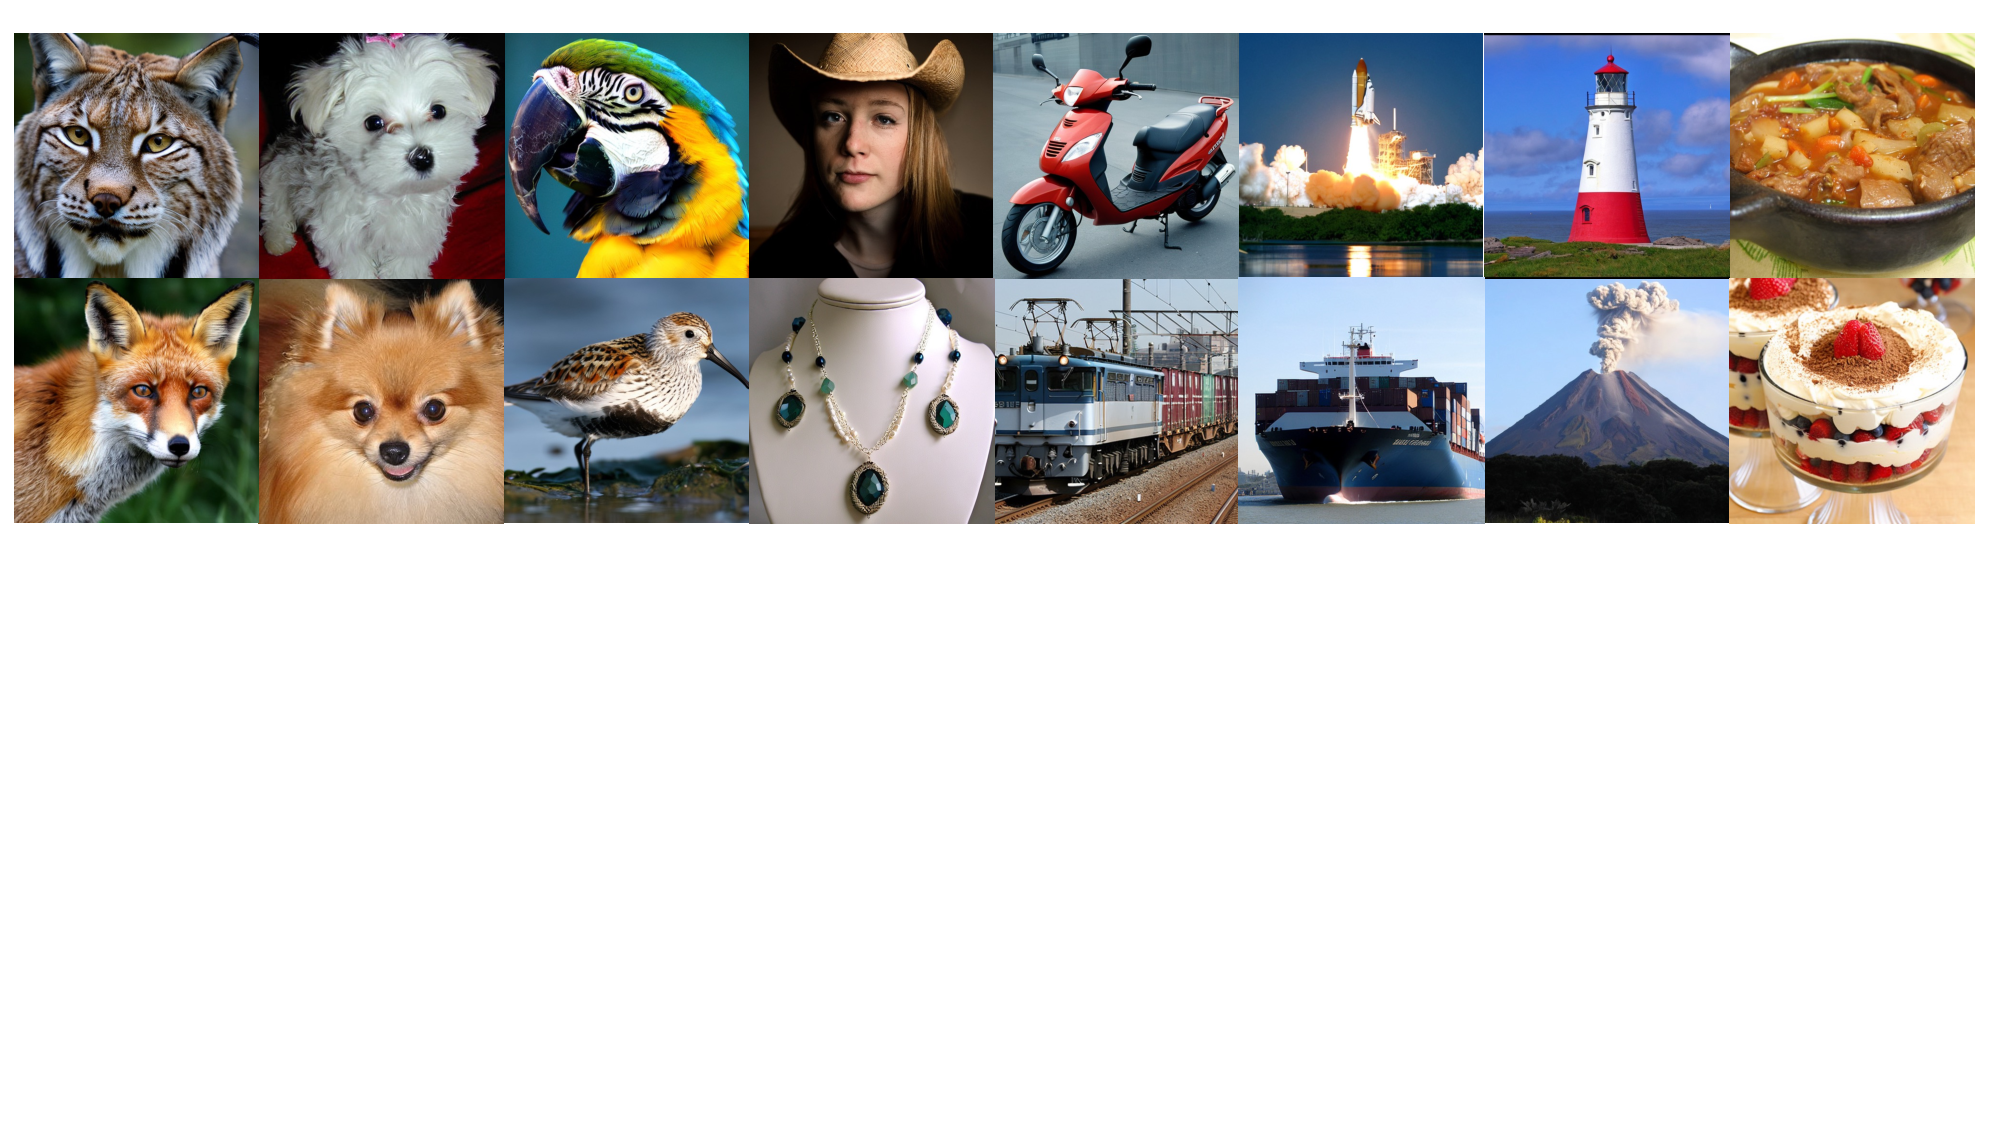
\includegraphics[width=\linewidth]{figs/figure2.pdf}
    \caption{Samples generated by CausalFusion-XL/2, ImageNet 512$\times$512, 800 epoch, DDPM 250 steps, CFG=4.0}
  \end{subfigure}
  \begin{subfigure}{1.0\linewidth}
    \centering
    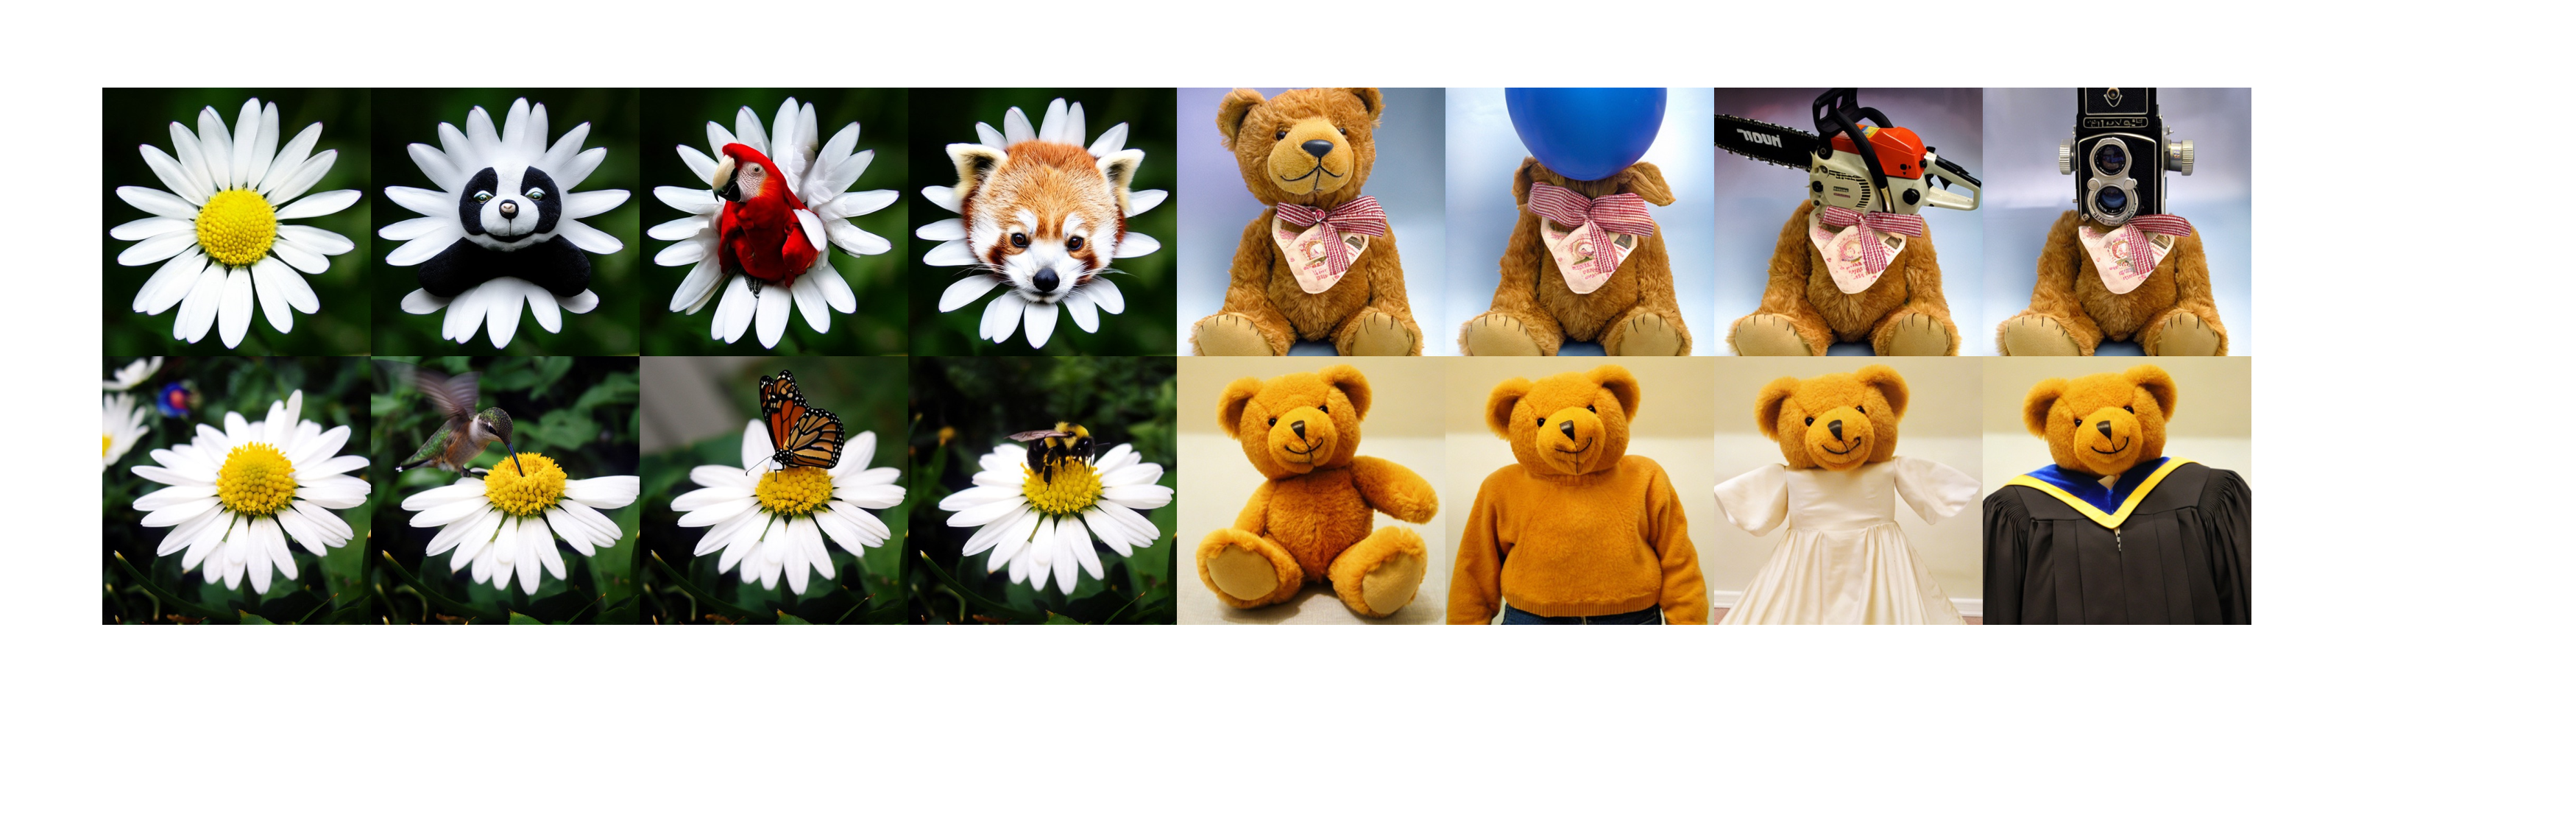
\includegraphics[width=\linewidth]{figs/edit.pdf}
    \caption{\textbf{Zero-shot image editing} results generated by CausalFusion-XL/2, ImageNet 512$\times$512, 800 epoch. We first generate the original image (those on the left), then mask out its centre region, top-half, or bottom-half, and regenerate the image with new class conditions. Details are discussed in Sec \ref{sec:system}.}
  \end{subfigure}
  \caption{\textbf{Visualization results}. All samples are generated by models trained only on \textbf{ImageNet-1K class-conditional generation} task, demonstrating CausalFusion's zero-shot image manipulation ability. See more visualization results in Appendix~\ref{appendix:secD}.
  \vspace{-12pt}
  }
  \vspace{-6pt}
  \label{fig:vis1}
\end{figure*}

The intrinsic distinction between AR and diffusion models lies in their approach to data distribution factorization. AR models treat data as an ordered sequence, factorizing it along the sequential axis, where the probability of each token is conditioned on all preceding tokens. This factorization enables the AR paradigm to generalize effectively and efficiently across arbitrary number of tokens, making it well-suited for long-sequence reasoning and in-context generation. In contrast, diffusion models factorize data along the noise-level axis, where the tokens at each step are a refined (denoised) version of themselves from the previous step. As a result, the diffusion paradigm is generalizable to arbitrary number of data refinement steps, enabling iterative quality improvement with scaled inference compute. While AR and diffusion models each excel within their respective domains, their distinct factorization approaches reveal complementary potential. Although recent studies~\cite{transfusion,monoformer,dart} have attempted to integrate AR and diffusion within a single model, they typically treat these paradigms as separate modes, missing the potential benefits of jointly exploring them within a 2-D factorization plane.

To this end, we introduce \textbf{CausalFusion}, a flexible framework that integrates both sequential and noise-level data factorization to unify their advantages. The degree of factorization along these two axes—namely, the AR step and diffusion step—is adjustable, enabling {CausalFusion} to revert seamlessly to the traditional AR or diffusion paradigms at either extreme. To enhance its generality, CausalFusion is designed to predict \textit{any} number of tokens at \textit{any} AR step, with \textit{any} pre-defined sequence order and \textit{any} level of inference compute, thereby minimizing the inductive biases presented in existing generative models. As shown in Figure~\ref{fig:dual-factorization}, this approach provides a broad spectrum between the AR and diffusion paradigms, allowing smooth interpolation within two endpoints during both training and inference. 
Specifically, we explore CausalFusion in image generation and multimodal generation scenarios, where we observe that the level of training difficulties significantly influences the overall effectiveness of CausalFusion.

\textbf{Difficulties of generative tasks in CausalFusion:} Both AR and diffusion paradigms present unique challenges based on difficulties of their specific generative stages. In diffusion models, the effectiveness of training depends heavily on proper loss weighting across noise levels~\cite{ddpm,minsnr}, as higher noise levels are more difficult and usually provide more valuable signals than lower noise levels. Similarly, AR models are susceptible to error accumulation~\cite{bengio2015scheduled} as early-stage predictions are made with limited visible context, making them more error-prone. Optimizing CausalFusion thus requires balancing across these varying task difficulties to optimize training signal impact and ensure sufficient exploration across the entire factorization plane.

In this paper, we formally examine the difficulties of generative tasks within CausalFusion. We show that, in addition to the noise levels in diffusion and the amount of visible context in AR, the total number of AR steps, which controls the interpolation between AR and diffusion, also plays a critical role in shaping training difficulties. Driven by these factors, we develop a scalable and versatile model based on the CausalFusion framework. Starting from the DiT architecture~\cite{dit}, we gradually convert it into a decoder-only transformer compatible with existing AR models like GPT~\cite{gpt1,gpt2,gpt3} and LLaMA~\cite{llama1,llama2,llama3}. We provide insights on how to appropriately choose the number of AR steps during the training of CausalFusion models, and further introduce loss weighing along both the diffusion and AR axis to balance the impact of different generative stages. As shown in Figure~\ref{fig:dual-factorization} and ~\ref{fig:vis1}, our model achieves state-of-the-art performance on the ImageNet class-conditional generation benchmark, significantly outperforming DiT~\cite{dit} and enabling zero-shot image manipulations due to its AR nature. When pretraining on both text-to-image and image-to-text tasks, our model surpasses forced-fusion frameworks such as TransFusion~\cite{transfusion}, demonstrating the versatility of our CausalFusion framework.


We highlight our main contribution below:
\begin{itemize}
\item  We propose CausalFusion as the AR counterpart to DiT, achieving state-of-the-art results and enabling the unlimited token generation for in-context reasoning.
\item  We systematically study CausalFusion on the dual-factorization plane and identify key factors that improve the effectiveness of CausalFusion models.
\item  Compared with recent studies~\cite{transfusion}, CausalFusion enables a smooth, cohesive integration with language modeling for cross-modal generation and reasoning.
\end{itemize} 
